\chapter{Convolutional Neural Networks (CNNs)}
Convolutional neural network are built on the foundamental principles of the ordinary MLPs, indeed both:
\begin{compactitemize}
    \item Are composed of neurons with learnable weights and biases.
    \item Receive inputs, perform dot products and often are follow it with a non-linearity activation function.
    \item Have the parameters organized in layers, end the entire network represent a single, differentiable function, crucial for the training via backpropagation.
\end{compactitemize}

\section{The parameter explosion problem in MLPs and the solution with CNNs}
When we use a MLP to process images, we have to flatten the image into a vector, and then feed it to the network. This approach increase the number of parameters dramatically.
\begin{examplebox}
    A small 32x32 pixel color image (32x32x3=3,072 input features) connected to a 512-neuron hidden layer would need over 1.5 million weights for that single layer! This is computationally expensive and prone to overfitting.
\end{examplebox}
Another two big problem of MLPs are:
\begin{compactitemize}
    \item \textbf{Loss of Spatial Information:} MLPs require flattening the image, into 1D vector. This process discards the spatial relationships between pixels, it fortgets that pixel are arranged in a grid.
    \item \textbf{Inability to Learn Hierarchies:} These networks struggle to recognize that features are built hierarchically. For example, pixel from edges, edges combine into shapes, adn shapes from objects.
\end{compactitemize}

CNNs are specifically designed for image inputs.
Their main purpose is to automatically and adaptively learn spatial hierarchies of features.
They achieve this by detecting simple patterns in early layers and building upon them to
recognize more complex patterns in deeper layers.

\begin{infobox}[Inspiration from Biology: The Visual Cortex]
    The brain’s visual cortex processes information in stages. 
    Neurons in early stages detect simple features like edges, lines, and colors. 
    Later stages combine these simple patterns to recognize more complex elements like textures, shapes, and eventually entire objects. 
    Crucially, individual neurons only respond to stimuli in a small, localized region of our visual field. 
    This biological principle inspires the efficiency and scalability of CNNs.
\end{infobox}
    
\section{Architecture}
 A CNN is composed of a series of layers, each with a specific function:
\begin{compactitemize}
   \item \textbf{Convolutional Layers}
   \item \textbf{Activation Functions}
   \item \textbf{Pooling Layers}
   \item \textbf{Fully Connected Layers}
\end{compactitemize}

\begin{figure}[H]
    \centering
    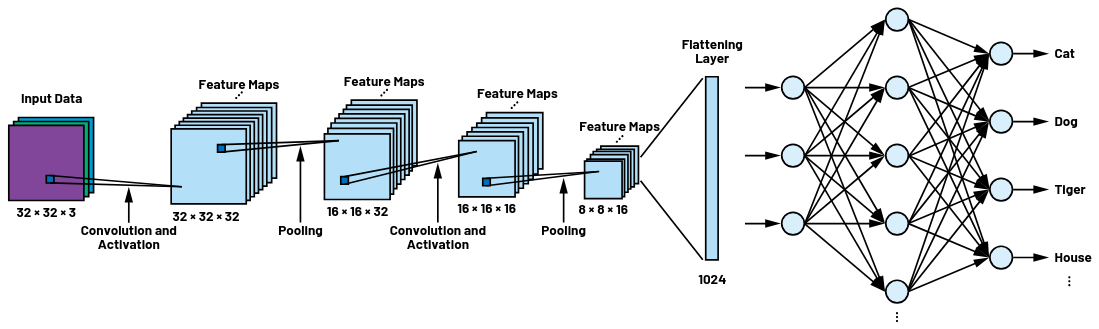
\includegraphics[width=1\textwidth]{images/CNN.png}
    \caption{Typical architecture of a Convolutional Neural Network (CNN).}
    \label{fig:cnn_architecture}
\end{figure}
Let's break down each component:
\begin{compactitemize}
    \item \textbf{The input:} The input to a CNN is typically a multi-channel image (e.g., RGB image with three channels). It is important to note that CNNs can also process other types of data, such as time series or 3D data, by adapting the convolutional operations accordingly.
    \item \textbf{Convolutional Layers:} These layers apply a set of learnable filters (or kernels) to the input image. Each filter slides over the input, performing a dot product between the filter and the local region of the input it covers. This operation produces a feature map that highlights specific patterns in the input, such as edges or textures. The filters are learned during training, allowing the network to adapt to the data.
    \item \textbf{Activation Functions:} After each convolutional operation, an activation function is applied to introduce non-linearity into the model. Common choices include ReLU (Rectified Linear Unit),sigmoid or tanh.
    \item \textbf{Pooling Layers:} These layers reduce the spatial dimensions of the feature maps, which helps to decrease the computational load and control overfitting. Common pooling operations include max pooling (which takes the maximum value in a local region) and average pooling (which computes the average value).
    \item \textbf{Fully Connected Layers:} After several convolutional and pooling layers, the high-level features are flattened into a 1D vector and passed through one or more fully connected layers. These layers function similarly to those in traditional MLPs, where each neuron is connected to every neuron in the previous layer. The final fully connected layer typically uses a softmax activation function for multi-class classification tasks.
\end{compactitemize}

\begin{infobox}[Important note]
    In the classic MLPs the feature extraction and the classification are both performed by the linear layers, while in CNNs the feature extraction is performed by the convolutional and pooling layers, and the classification is performed by the fully connected layers. It also important to note that like in MLPs, the firt layers was bigger and the last layer was smaller, in the first convolutional layer we tend to have more filters, while in the last convolutional layer we tend to have less filters. This is valid also for the spatioal dimensions, in the first convolutional layer we tend to have a bigger spatial dimension, while in the last convolutional layer we tend to have a smaller spatial dimension. This is made beacuse we want give in input to the fully connected layers a small number of features possible.
\end{infobox}

\section{Convolutional Layers}
Identically to the MLPs what a neuron does is a simple weighted sum of its input plus a bias:
\[
y = \sum_{i=1}^{n} w_i x_i + b
\]

\begin{tcolorbox}[
    colback=white,    % sfondo bianco (puoi anche mettere "colback=none")
    colframe=white,   % bordo invisibile
    boxrule=0pt,      % spessore bordo = 0
    arc=0pt,          % angoli non arrotondati (opzionale)
    left=0pt, right=0pt, top=0pt, bottom=0pt, % nessun margine interno extra
    enlarge left by=0mm, enlarge right by=0mm % allineamento perfetto
]
\begin{minipage}{0.65\textwidth}
However, a key difference in convolutional layers is that neurons are only \textbf{locally connected} to a small contiguous region of the input volume. 
This small region that each neuron "sees" of the previous layer is called the \textbf{receptive field} of the neuron. 
The size of the receptive field increases with the depth of the network: as we go deeper in the network, each neuron will see a larger portion of the input image, even if the size of the kernel remains the same.
\end{minipage}\hfill
\begin{minipage}{0.3\textwidth}
\centering
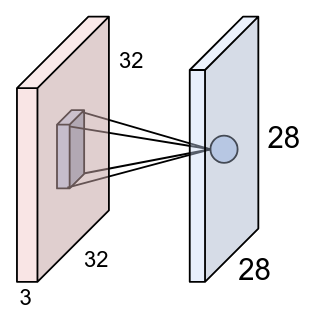
\includegraphics[width=\linewidth]{images/local_connettivity.png}
\captionof{figure}{Local connectivity in CNNs.}
\end{minipage}
\end{tcolorbox}

\begin{infobox}[Intuition of parameter sharing]
    Intuition: If a feature (e.g., an edge or a specific texture) is useful to detect at one spatial
    location in an image, it’s likely useful to detect it at other locations too.
    To leverage this, we constrain all neurons within a single depth slice (i.e., those producing a
    single feature map) to share the same set of weights and bias.
    This parameter sharing allows the forward pass of a convolutional layer to be computed as a
    convolution operation. Each set of shared weights is often referred to as a filter or kernel
    that scans across the entire input volume.
\end{infobox}

Suppose that one kernel catch a specific feature, we may use more kernel to catch more features, so we can have multiple filters in a convolutional layer. In particular during the forward pass:

\begin{compactitemize}
    \item Each filter is \textbf{convolved} with the input volume.
    \item This operation produces a 2D output, called a \textbf{feature map} or \textbf{activation map}.
    \item A distinc feature map is generated for each filter.
\end{compactitemize}
The output volume of a convolutional layer is obtained by stacking the feature maps produced by each filter along the depth dimension.

\begin{figure}[H]
    \centering
    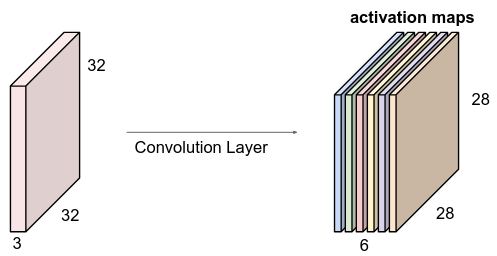
\includegraphics[width=0.45\textwidth]{images/CNN_layer.png}
    \caption{Convolutional layer with multiple filters producing multiple feature maps.}
    \label{fig:cnn_multiple_filters}
\end{figure}
When we talk about a kernel size, we reffere always to the spatial dimensions of the kernel, so a kernel size of 3x3 means that the kernel has a height and width of 3 pixels each. The depth of the kernel is always equal to the depth of the input volume. So for example with a input 5x5x3 the parameter to learn are 75 not 25.

\subsection{What is the convolution operation?}
The convolution operation is a mathematical operation that combines two functions to produce a third function. In the context of CNNs, it involves sliding a filter (or kernel) over the input image and computing the dot product between the filter and the local region of the input it covers. This operation is repeated across the entire input image to produce a feature map.
The convolution operation can be mathematically expressed as:
\[
S(i, j) = (I * K)(i, j) = \sum_{m} \sum_{n} I(i+m, j+n) K(m, n)
\]
Where:
\begin{compactitemize}
    \item \(S(i, j)\) is the output feature map at position \((i, j)\).
    \item \(I\) is the input image.
    \item \(K\) is the filter (or kernel).
    \item \(m\) and \(n\) are the dimensions of the filter.
\end{compactitemize}
\begin{figure}[H]
    \centering
    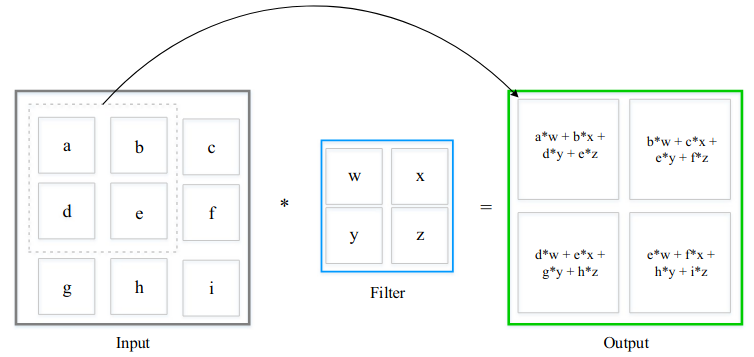
\includegraphics[width=0.8\textwidth]{images/convolution.png}
    \caption{Convolution operation example.}
    \label{fig:convolution_operation}
\end{figure}
\textbf{Note:} that this diagram simplifies the proccess for a single channel. In reality, a filter's depth must match the input volume's depth (e.g., a 3x3x\textbf{3} filter fot a 32x32x\textbf{3} input image). The convolution involves element-wise multiplication across all channels, and the result are summed up, along with a bias term, to produce a single value in the output feature map.

\subsection{Hyperparameters of Convolutional Layers}
Each convolutional layer is defined by the following hyperparameters:
\begin{compactitemize}
    \item \textbf{Number of Filters ($C_{\text{out}}$)}: Determines the depth of the output volume (i.e., how many feature maps are produced).
    \item \textbf{Kernel Size ($K \times K$)}: The spatial dimensions of the convolutional filters. These are typically square. Each filter also extends through the full depth ($C_{\text{in}}$) of the input volume.
    \item \textbf{Stride ($S$)}: The number of pixels the convolutional filter shifts across the input at each step. A larger stride results in a smaller output volume.
\end{compactitemize}
Additionally, the presence and amount of \textbf{Spatial Padding ($P$)} applied to the input volume can be considered another hyperparameter. Padding is often used to preserve spatial dimensions or to ensure an integer output size.

\begin{infobox}[Different Types of Padding]
    When we talk about padding, the first question that arises is: with which value should we pad the input? The most common choice is to pad with zeros, a technique called \textbf{zero-padding}. Zero-padding is simple and computationally efficient, and it allows us to control the spatial dimensions of the output volume. However, it can also introduce some artifacts: the artificial addition of zeros creates "black regions" along the borders of the feature maps, which do not represent any real information from the input. These regions can sometimes bias the network, especially in early layers, causing the convolutional filters to respond differently near the edges compared to the center of the input.  
    
    To mitigate these issues, other padding strategies can be used. \textbf{One-padding} consists of filling the padded areas with ones instead of zeros. This can reduce the stark contrast created by zeros, but it may still introduce artificial patterns that the network could misinterpret. Another approach is \textbf{mirror-padding}, also called \textbf{reflect-padding}, where the border values of the input are mirrored to extend the input volume. This technique helps preserve the local structures and patterns at the edges, minimizing artificial bias while still allowing control over output dimensions. Each padding strategy has its trade-offs, and the choice often depends on the type of data and the specific architecture being used.
\end{infobox}

\subsection{Number of Learnable Parameters}
Given an input volume of size \(H_{\text{in}} \times W_{\text{in}} \times C_{\text{in}}\) and a convolutional layer with \(C_{\text{out}}\) filters of size \(K \times K\), the number of learnable parameters in the convolutional layer can be calculated as follows:
\[
\text{Number of Parameters} = (K \times K \times C_{\text{in}} + 1) \times C_{\text{out}}
\]
Where:
\begin{compactitemize}
    \item \(K \times K \times C_{\text{in}}\) is the number of weights per filter (the filter size times the depth of the input volume).
    \item The "+1" accounts for the bias term associated with each filter.
    \item \(C_{\text{out}}\) is the number of filters in the convolutional layer.
\end{compactitemize}

\begin{figure}[H]
    \centering
    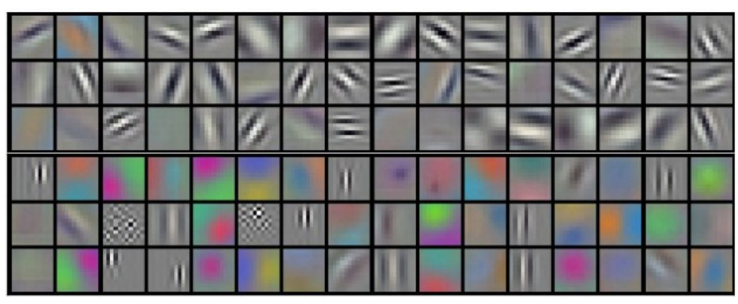
\includegraphics[width=0.8\textwidth]{images/filter_example.png}
    \caption{Examples of learned weight from the first convolutional layer.}
    \label{fig:cnn_learned_weights}
\end{figure}

Each of the 96 filters shown here is of size 11 × 11 × 3. This visualization confirms that the
parameter sharing assumption is highly reasonable: if detecting a feature like a horizontal edge
is important at one location in an image, it’s intuitively useful at other locations as well,
contributing to the \textbf{translational invariance} of CNNs.

\subsection{Activation Functions}
Activation functions introduce critical non-linearity into the network by performing an element-wise operation on the input volume. The most common ones include:

\begin{figure}[H]
    \centering
    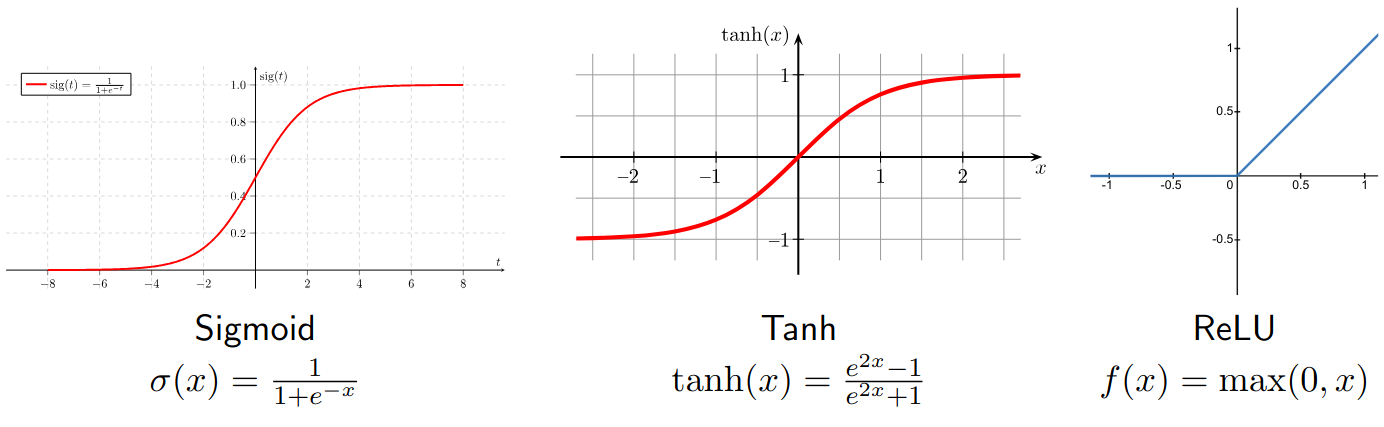
\includegraphics[width=1\textwidth]{images/activation_function.png}
    \caption{Most common activation functions used in CNNs.}
    \label{fig: activation_functions}
\end{figure}
It's worth noting that more advances activation functions have also been developed.

Among these activation function the most widely used is the relu, this is because:
\begin{compactitemize}
    \item \textbf{Accelerated Convergence:} ReLU was empirically found to greatly accelerate the convergence of SGD compared to sigmoid/tanh in many scenarios.
    \item \textbf{Computational Efficiency:} ReLU can be implemented by a simple thresholding operation ($f(x)=max(0,x)$), wheread Sigmoid and Tanh involve more complex exponential calculations.
\end{compactitemize}

Follow is shown a visulizating activation maps from different CNN stages (layer). To show the network's area focus, each map is upsampled to match the original image's dimension.
\begin{figure}[H]
    \centering
    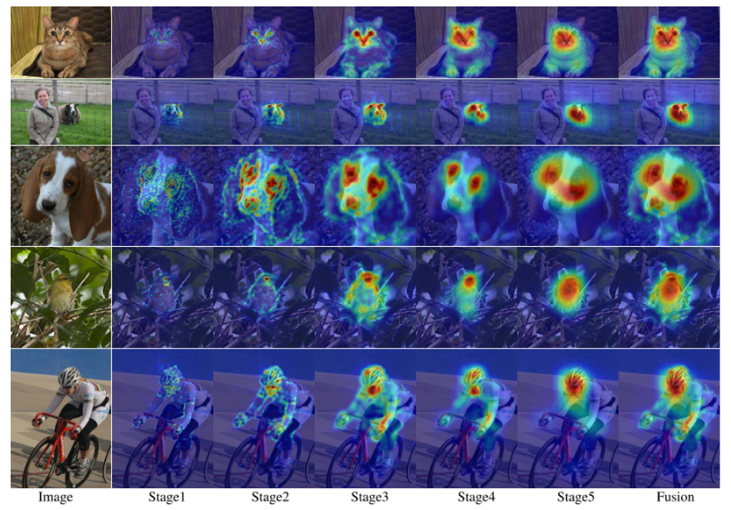
\includegraphics[width=0.6\textwidth]{images/stage.png}
    \caption{Activation maps from different CNN stages.}
    \label{fig: cnn_stages}
\end{figure}

\section{Pooling Layers}
Pooling layers are used to reduce the spatial dimensions (height and width) of the input volume, while retaining the most important information. This downsampling helps to decrease the computational load, control overfitting, and make the network more robust to small translations in the input.
\begin{figure}[H]
    \centering
    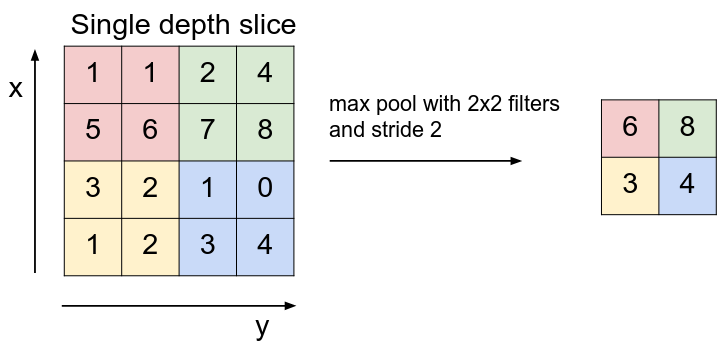
\includegraphics[width=0.5\textwidth]{images/max_pooling.png}
    \caption{Max pooling operation example.}
    \label{fig:max_pooling_operation}
\end{figure}

Key hyperparameters of pooling layers include:
\begin{compactitemize}
    \item \textbf{Pool Size ($P \times P$)}: The spatial dimensions of the pooling window. Common choices are 2x2 or 3x3.
    \item \textbf{Stride ($S$)}: The number of pixels the pooling window shifts across the input at each step. A larger stride results in a smaller output volume. When $S=K$, the pooling windows do not overlap.
\end{compactitemize}

The type of \textbf{pooling function} used is an addition to hyperparameter. While many aggregation functions are possible, the mosto common in practice are:
\begin{compactitemize}
    \item \textbf{Max Pooling:} Takes the maximum value within the pooling window. This operation is effective at capturing the most prominent features and is widely used in practice.
    \item \textbf{Average Pooling:} Computes the average value within the pooling window. This approach provides a smoother representation of the features but may dilute strong activations.
\end{compactitemize}

\begin{infobox}[Typical Pooling Configuration]
    The tipically configuration of a pooling layer is a 2x2 max pooling with stride 2. In this setting, $75$ of input volume activation are discarded.
\end{infobox}

\begin{infobox}[Pooling layer cons]
    While beneficial for some tasks, the aggressive downsampling of pooling layers can lead to a loss of spatial information, which may be detrimental for tasks requiring precise localization, such as image segmentation. Additionally, pooling operations are not learnable, meaning they do not adapt to the data during training. This limitation has led to the exploration of alternative downsampling methods, such as strided convolutions or adaptive pooling techniques, which can provide more flexibility and potentially better performance in certain applications.
\end{infobox}

\begin{figure}[H]
    \centering
    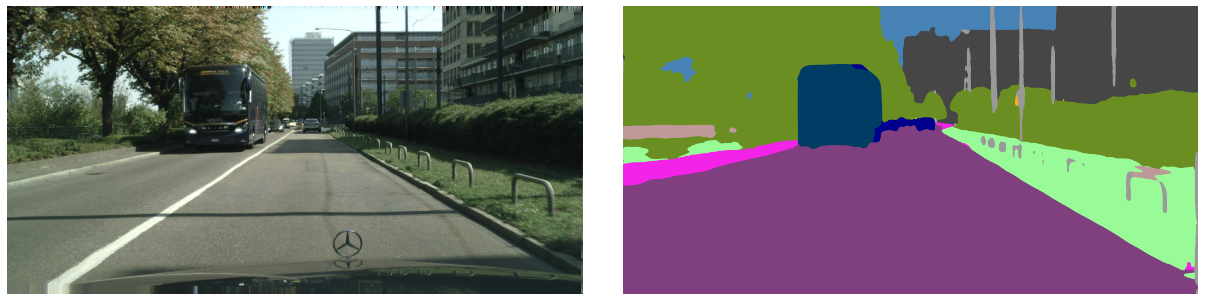
\includegraphics[width=0.9\textwidth]{images/loss_spatial.png}
    \caption{Loss of spatial information due to pooling.}
    \label{fig:loss_spatial_info}
\end{figure}

\subsection{Computing Output Volume Size}
Initially, let's define the variables:
\begin{compactitemize}
    \item \(H_{\text{in}}\): Height of the input volume.
    \item \(W_{\text{in}}\): Width of the input volume.
    \item \(C_{\text{in}}\): Depth (number of channels) of the input volume.
    \item \(C_{\text{out}}\): Number of filters (depth of the output volume).
    \item \(K\): Kernel size
    \item \(S\): Stride 
    \item \(P\): Padding
\end{compactitemize}

For a \textbf{convolutional layer}, given an input volume of size \(H_{\text{in}} \times W_{\text{in}} \times C_{\text{in}}\), the output volume size can be computed as follows:
\[
H_{\text{out}} = \frac{H_{\text{in}} - K + 2P}{S} + 1
\]
\[
W_{\text{out}} = \frac{W_{\text{in}} - K + 2P}{S} + 1
\]
\[
C_{\text{out}} = \text{Number of filters}
\]

For a \textbf{pooling layer}, given an input volume of size \(H_{\text{in}} \times W_{\text{in}} \times C_{\text{in}}\), the output volume size can be computed as follows:
\[
H_{\text{out}} = \frac{H_{\text{in}} - P}{S} + 1
\]
\[
W_{\text{out}} = \frac{W_{\text{in}} - P}{S} + 1
\]
\[
C_{\text{out}} = C_{\text{in}}
\]

For an \textbf{activation layer}, the output volume size remains the same as the input volume size:
\[
H_{\text{out}} = H_{\text{in}}
\]
\[
W_{\text{out}} = W_{\text{in}}
\]
\[
C_{\text{out}} = C_{\text{in}}
\]
This is because activation functions are applied element-wise and do not change the spatial dimensions or depth of the volume.

\section{Real Implementation of CNNs}

\subsection{LeNet}
The architecture known as \textbf{LeNet} was introduced in one of the pioneering works on Convolutional Neural Networks (CNNs), laying much of the groundwork for modern deep learning approaches. It demonstrated the \textbf{efficacy of CNNs for handwritten digit recognition} through an end-to-end trainable design. The network processes \textbf{32×32 pixel input images} through successive layers of convolution and subsampling, where each convolutional layer employs \textbf{learnable filters (5×5 kernels)} to extract spatial features. The subsampling layers, using \textbf{average pooling over 2×2 windows with stride 2}, progressively reduce spatial resolution while preserving essential information. Non-linear transformations are introduced through \textbf{sigmoid activation functions}, whose coefficients and biases control the non-linearity of each unit. This architecture alternates convolutional and subsampling layers, forming a bi-pyramidal structure in which the \textbf{number of feature maps increases as spatial resolution decreases}. Overall, LeNet represented one of the first \textbf{complete, trainable CNN architectures}, setting the foundation for subsequent developments in deep learning.
\begin{figure}[H]
    \centering
    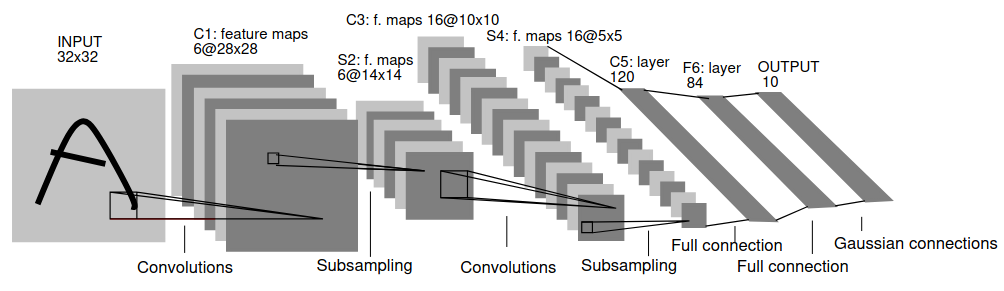
\includegraphics[width=0.9\textwidth]{images/LeNet.png}
    \caption{LeNet architecture.}
    \label{fig:lenet_architecture}
\end{figure}

\subsection{AlexNet}
\textbf{AlexNet}, introduced in 2012, marked a major breakthrough in image recognition by winning the \textbf{ImageNet Large Scale Visual Recognition Challenge} with a significant margin, demonstrating the unprecedented power of \textbf{Convolutional Neural Networks (CNNs)} at scale. The architecture consisted of \textbf{eight layers with learnable parameters}, including five convolutional and three fully connected layers, processing high-dimensional image inputs. The network employed a \textbf{large first kernel (11×11)} in its initial convolutional layer, enabling the capture of broader spatial context. Moreover, AlexNet \textbf{pioneered the use of Rectified Linear Units (ReLU)} as activation functions, which significantly accelerated training compared to traditional sigmoidal activations. Another key innovation was the \textbf{parallel training across two GPUs}, allowing the model to handle an unprecedented number of parameters for its time, with limited inter-GPU communication at specific layers. Overall, AlexNet established the foundation for the deep learning revolution in computer vision.
\begin{figure}[H]
    \centering
    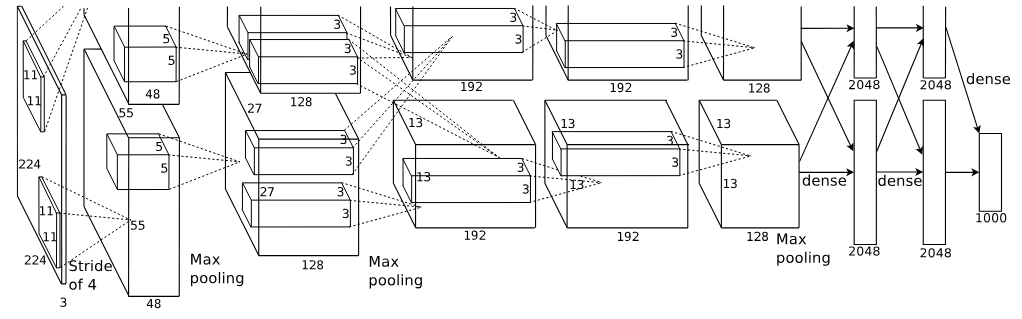
\includegraphics[width=0.9\textwidth]{images/AlexNet.png}
    \caption{AlexNet architecture.}
    \label{fig:alexnet_architecture}
\end{figure}

\subsection{VGGNet}
\textbf{VGG}, introduced in 2014 by the \textbf{Oxford Visual Geometry Group (VGG)}, represents a family of deep convolutional neural networks that achieved remarkable success in large-scale image recognition tasks. It became widely recognized for its \textbf{simplicity, effectiveness, and influence} on subsequent network designs. The model \textbf{secured 1st and 2nd places} in the ImageNet 2014 localization and classification challenges, establishing a new standard for deep learning architectures.  
\begin{compactitemize}
    \item \textbf{Input:} Fixed-size \(224 \times 224\) RGB images, mean-subtracted during pre-processing.  
    \item \textbf{Architecture:} Consists of 16 weight layers (\textbf{VGG16}), including 13 convolutional and 3 fully connected layers.  
    \item \textbf{Convolutional Filters:} Employs small and uniform \textbf{3×3 kernels} with stride 1, stacked to increase non-linearity and capture complex patterns effectively.  
    \item \textbf{Activation Function:} Each convolutional and fully connected layer is followed by a \textbf{ReLU} activation function.  
    \item \textbf{Spatial Pooling:} Includes five \textbf{max-pooling layers} using 2×2 windows with stride 2 for progressive spatial downsampling.  
    \item \textbf{Fully Connected Layers:} The last three layers are fully connected, with the first two containing \textbf{4096 neurons} each and the final one having \textbf{1000 neurons} for classification, followed by a \textbf{Softmax} activation.  
    \item \textbf{Pre-trained Weights:} Released publicly, enabling \textbf{transfer learning} and establishing VGG as a popular backbone for diverse computer vision tasks.    
\end{compactitemize}
\begin{figure}[H]
    \centering
    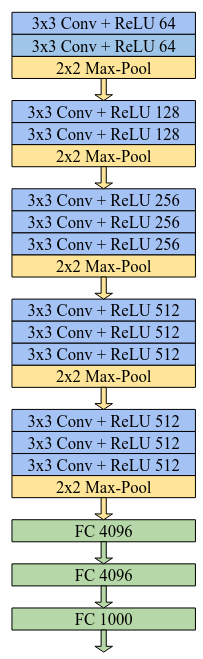
\includegraphics[height=0.4\textheight,keepaspectratio]{images/VGG.png}
    \label{fig:forecast_prediction}
\end{figure}

The net contains approximately \textbf{138 million learnable parameters}, with about \textbf{70\% located in the fully connected layers}. Notably, a single fully connected layer is responsible for roughly \textbf{100 million parameters}.
\begin{figure}[H]
    \centering
    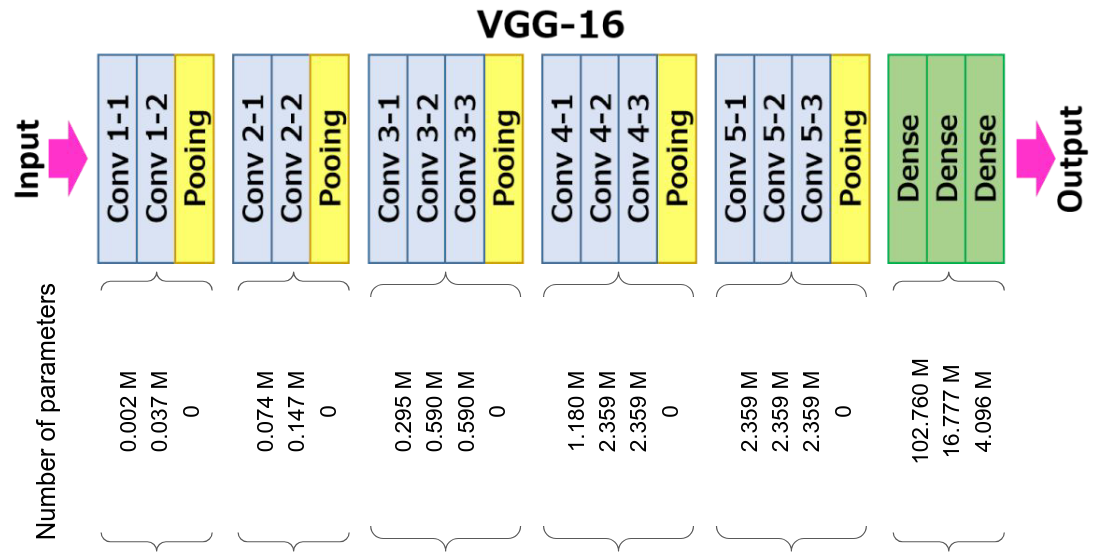
\includegraphics[width=0.7\textwidth]{images/number_parameters.png}
    \caption{Number of parameters in VGG16.}
    \label{fig:vgg_number_parameters}
\end{figure}
In traditional convolutional neural networks, simply \textbf{stacking more layers beyond a certain depth} often leads to \textbf{performance degradation} rather than improvement. This phenomenon is \textbf{not caused by overfitting}, as deeper models exhibit \textbf{higher training and test error}. A key hypothesized reason is the \textbf{difficulty of training deep layers to approximate simple identity mappings}. Additionally, very deep networks suffer from the problem of \textbf{vanishing or exploding gradients}, where gradients propagated backward through many layers become either extremely small (\textbf{vanishing}) or extremely large (\textbf{exploding}). This instability severely \textbf{hinders the ability of early layers to learn effectively}, making it challenging to train very deep architectures.

\subsection{The state of the art: The Residual Neural Network (ResNet)}
\textbf{ResNet (Residual Networks)}, introduced in 2015, was a groundbreaking architecture that won both the \textbf{ImageNet Large Scale Visual Recognition Challenge (ILSVRC 2015)} and \textbf{COCO 2015} for detection, segmentation, and localization. ResNet addressed the critical problem of training very deep convolutional networks, which often suffered from performance degradation due to \textbf{vanishing or exploding gradients}.  
\begin{figure}[H]
    \centering
    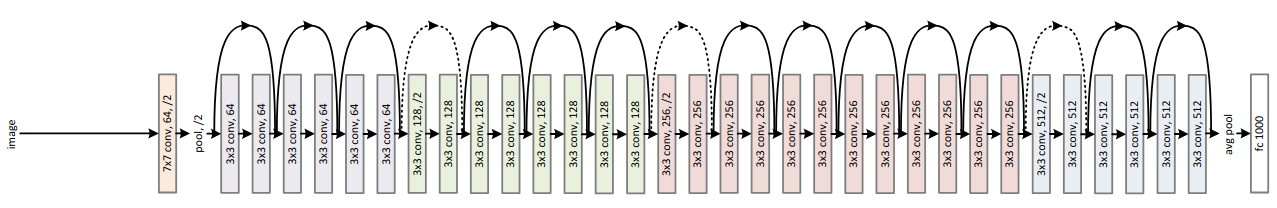
\includegraphics[width=1\textwidth]{images/ResNet.png}
    \caption{ResNet architecture.}
    \label{fig:resnet_architecture}
\end{figure}
\begin{compactitemize}
    \item \textbf{Input:} Accepts \(224 \times 224\) RGB images.
    \item \textbf{Architecture:} Features \textbf{ultra-deep networks}, with common variants including \textbf{ResNet-50, ResNet-101, and ResNet-152}, reaching up to 152 layers, far deeper than VGG.  
    \item \textbf{Output:} Produces predictions for \textbf{1000 ImageNet classes}.  
    \item \textbf{Key Innovation – Residual Learning:} Instead of directly learning the underlying mapping \(H(x)\), the network learns the \textbf{residual function} \(F(x)\) such that:
    \[
    H(x) = F(x) + x
    \]
    This formulation allows layers to focus on learning the difference (residual) between the desired output and the input, making optimization easier.  
    \item \textbf{Residual Block:} The fundamental building block of ResNet, implemented via \textbf{skip connections}:
    \begin{itemize}
        \item The input \(x\) is added directly to the output of the residual function \(F(x)\).  
        \item \textbf{Easier gradient flow:} Skip connections allow gradients to bypass intermediate layers, mitigating vanishing/exploding gradient problems.  
        \item Supports much deeper networks without performance degradation.  
    \end{itemize}
    \begin{figure}[H]
        \centering
        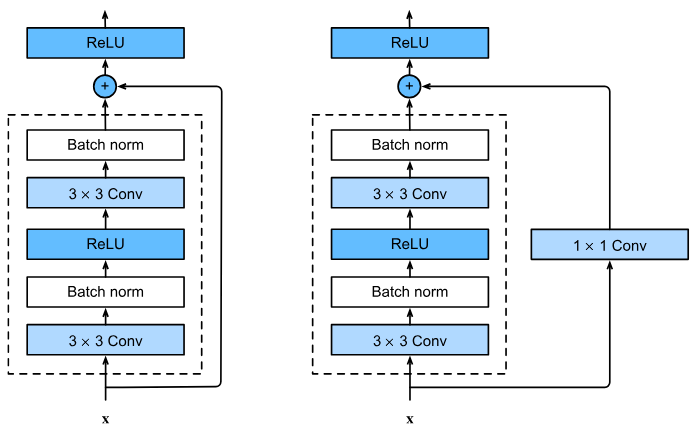
\includegraphics[width=0.5\textwidth]{images/residual_block.png}
        \caption{Residual Block.}
        \label{fig:residual_block}
    \end{figure}
    \item \textbf{Impact and Advantages:}
    \begin{itemize}
        \item \textbf{Enabled ultra-deep networks:} Training models with unprecedented depth (e.g., 152 layers) became feasible.  
        \item \textbf{Improved performance:} Achieved state-of-the-art results across numerous computer vision tasks, including image classification, detection, and segmentation.  
        \item \textbf{Simplified training:} Residual connections reduce optimization difficulty, preventing the degradation problem observed in traditional deep networks.  
        \item \textbf{Foundation for future architectures:} The concept of \textbf{skip connections} and residual learning influenced many subsequent CNN architectures and even modern Transformer models.  
    \end{itemize}
\end{compactitemize}

\section{Batch Normalization}
In deep neural networks with many layers, the distribution of inputs to each layer tends to change continuously during training as the parameters of the preceding layers are updated. This phenomenon is known as \textbf{Internal Covariate Shift}. It occurs because every time the weights in earlier layers are modified, the statistical properties (mean and variance) of the inputs received by deeper layers also change. As a result, each layer must constantly adapt to a shifting input distribution, which \textbf{slows down training} and makes it more difficult for the network to converge effectively. Small parameter changes in the early layers can become amplified as they propagate forward through the network, leading to instability and poor optimization efficiency.  
\begin{figure}[H]
    \centering
    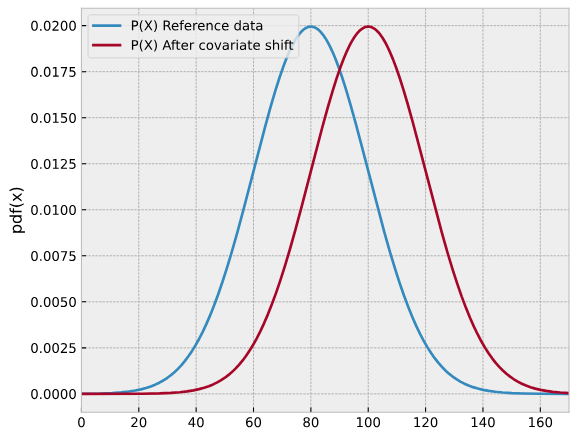
\includegraphics[width=0.5\textwidth]{images/covariance_shift.png}
    \caption{Internal covariance shift.}
    \label{fig:internal_covariance_shift}
\end{figure}
To address this issue, \textbf{Batch Normalization (BN)} was introduced in the paper \textit{"Batch Normalization: Accelerating Deep Network Training by Reducing Internal Covariate Shift"} by Ioffe and Szegedy (2015). Batch Normalization standardizes the inputs to each layer within a mini-batch by re-centering and rescaling them to have zero mean and unit variance, followed by a learnable shift and scale transformation. This normalization \textbf{stabilizes the learning process}, allowing higher learning rates, faster convergence, and reduced sensitivity to weight initialization. By mitigating internal covariate shift, Batch Normalization made the training of very deep networks significantly more stable and efficient, becoming a fundamental component of modern deep learning architectures.

\subsection{How Batch Normalization Works During Training}
During training, Batch Normalization operates on mini-batches of data to normalize the inputs to each layer. The process involves the following steps for each mini-batch:
\begin{compactitemize}
    \item \textbf{Compute Batch Statistics:} For each feature in the mini-batch, calculate the mean (\(\mu_B\)) and variance (\(\sigma_B^2\)):
    \[
    \mu_B = \frac{1}{m} \sum_{i=1}^{m} x_i
    \]
    \[
    \sigma_B^2 = \frac{1}{m} \sum_{i=1}^{m} (x_i - \mu_B)^2
    \]
    where \(m\) is the number of examples in the mini-batch, and \(x_i\) represents the input features.
    \item \textbf{Normalize the Inputs:} Each input feature is normalized using the computed mean and variance:
    \[
    \hat{x}_i = \frac{x_i - \mu_B}{\sqrt{\sigma_B^2 + \epsilon}}
    \]
    where \(\epsilon\) is a small constant added for numerical stability.
    \item \textbf{Scale and Shift:} The normalized inputs are then scaled and shifted using learnable parameters \(\gamma\) (scale) and \(\beta\) (shift):
    \[
    y_i = \gamma \hat{x}_i + \beta
    \]
    This allows the network to learn an optimal representation of the data after normalization.
\end{compactitemize}
After normalizing, the activations have a mean of 0 and a standard deviation of 1. This might be too restrictive for the network. To address this, Batch Normalization introduces two learnable parameters per feature: a scaling factor \(\gamma\) and a shifting factor \(\beta\). These parameters allow the network to adjust the normalized output, enabling it to recover the original distribution if necessary. By learning these parameters, the network can maintain its expressive power while benefiting from the stability provided by normalization.

\subsection{How Batch Normalization Works During Inference}
During inference (testing or deployment), the behavior of Batch Normalization differs from training. Instead of using the statistics computed from the current mini-batch, Batch Normalization relies on \textbf{running estimates} of the mean and variance that were accumulated during training. The steps are as follows:
\begin{compactitemize}
    \item \textbf{Use Running Estimates:} Instead of calculating the mean and variance from the current mini-batch, use the running estimates \(\mu_{\text{running}}\) and \(\sigma_{\text{running}}^2\) that were updated during training.
    \item \textbf{Normalize the Inputs:} Each input feature is normalized using the running estimates:
    \[
    \hat{x}_i = \frac{x_i - \mu_{\text{running}}}{\sqrt{\sigma_{\text{running}}^2 + \epsilon}}
    \]
    \item \textbf{Scale and Shift:} The normalized inputs are then scaled and shifted using the learned parameters \(\gamma\) and \(\beta\):
    \[
    y_i = \gamma \hat{x}_i + \beta
    \]
\end{compactitemize}
This approach ensures that the model's predictions are consistent and stable during inference, as they are based on the overall data distribution learned during training rather than the potentially noisy statistics of a single mini-batch.

\subsection{Benefits of Batch Normalization}
Batch Normalization offers several significant benefits that enhance the training and performance of deep neural networks:
\begin{compactitemize}
    \item \textbf{Faster Training:} Allows for higher learning rates, leading to quicker convergence and reduced training time.
    \item \textbf{Reduces Internal Covariate Shift:} Stabilizes the distribution of layer inputs, making the training process more stable.
    \item \textbf{Regularization Effect:} The noise from mini-batch statistics has a slight regularizing effect, sometimes reducing the need for dropout.
    \item \textbf{Less Sensitive to Inizialization:} Makes the network less dependent on the initial weights.
\end{compactitemize}